\documentclass[11pt]{article}
\usepackage{xeCJK}
\setCJKmainfont{Noto Serif CJK TC}%引入fonts
\usepackage[top=2cm,bottom=2cm,left=3cm,right=3cm,a4paper]{geometry}%edges
\usepackage{setspace}
\onehalfspacing
\setlength{\parskip}{6pt}%gap
\usepackage{moresize}
\usepackage{graphicx}
\usepackage{xcolor}
%%%%%%%%%%%%%%%%%%%%%%%%%%Get Started%%%%%%%%%%%%%%%
\begin{document}
\begin{titlepage}
\begin{center}
\vspace*{4cm}
\LARGE    禁書目錄\\
\HUGE  \textbf{三角函數本}\\
\vspace{0.5cm}
\small    Index Librorum Prohibitorum\\
\normalsize  \textbf{Trigo functions}\\[1cm]
\Large Paco Index\\[0.5cm]
\Large Last updated: 23 Jan 2025\\[1.5cm]

\includegraphics[width=6cm]{images/INDEX.PNG}\\[3cm]
\LARGE Eli, Eli, lema sabachthani?\\
\large 主!為什麼離棄我?
\small 《聖經·馬太福音》
\vfill
\end{center}
\end{titlepage}
\section*{\Huge Chapter 1 任意角與弧度制}
\vspace{0.25cm}
\subsection*{\LARGE 1.1 角}{
    \large \textbf{Definition:}\\
    一條射綫繞其端点逆時針方向旋轉形成的角叫\textcolor{red}{正角}\\
    反之,順時針方向旋轉形成的角叫\textcolor{red}{負角}\\
    若它沒有做任何旋轉,我們則稱它為\textcolor{red}{零角}\\
    \begin{figure}[h]
    \centering
    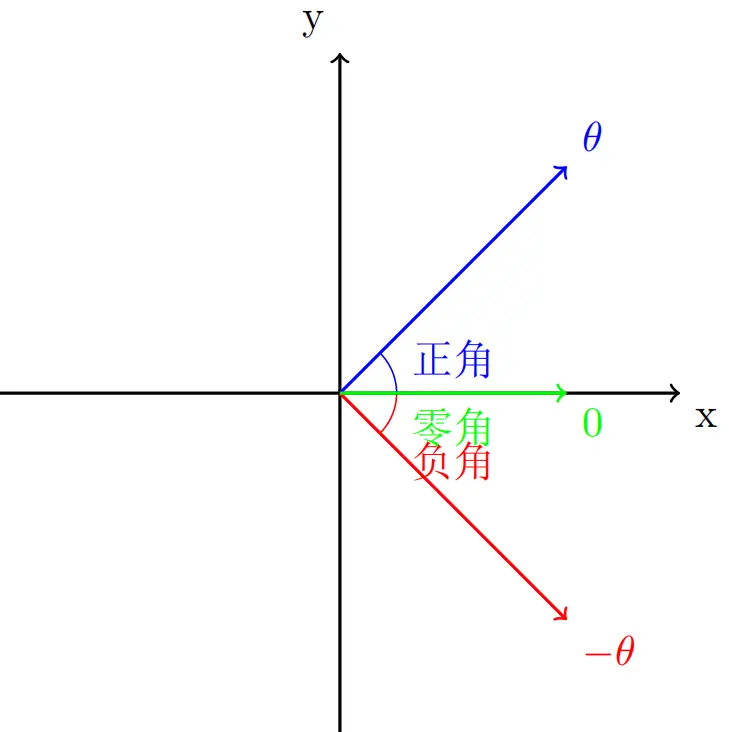
\includegraphics[width=5cm]{images/pos-neg-an.png}\\
    \caption{}
    \label{fig:enter-label}
    \end{figure}
}\\
不難知,若我們想得到$\alpha+\beta$角,可以先逆時針旋轉$\alpha$,再逆時針旋轉$\beta$.\\
同理,若我們想得到$\alpha-\beta$角,可以先逆時針旋轉$\alpha$,再順時針旋轉$\beta$\textcolor{red}{(即逆時針旋轉($-\beta$))}.\\

我們也注意到了任何角旋轉$360^{\circ}$後,其終辺位置不變.
故我們知\textcolor{blue}{所有與$\alpha$終辺相同的角的集合為$S=\{\theta:\theta=\alpha+k\cdot360^{\circ},k\in \mathbf{Z}\}$}
\subsection*{\LARGE 1.2 弧度制}{
    \large \textbf{Definition:}\\
    長度等於半徑長的圓弧所対的圓心角,叫做弧度1 rad的角(rad 通常忽略不寫)\\

    上述Definition其實並不好用,我們其實可以理解成:
    在半徑為$r$的圓中,圓心角$\alpha$所対圓弧$l$.
    那麼便有:$$|\alpha|=\frac{l}{r}$$\\
    故一個單位圓中,我們易知:$360^{\circ}=2\pi$$\Rightarrow$\textcolor{blue}{$180^{\circ}=\pi$}\\[5cm]
    \large \textbf{度數與弧度的轉換:}\\
    以度數表示的角,把數字乘以$\frac{\pi}{180^{\circ}}$便轉換成弧度;以弧度表示的角,乘以${\frac {180^{\circ }}{\pi }}$便轉換成度數。\\[0.5cm]
    \large \textbf{Example:}\\
    \large $60^{\circ}=60^{\circ}\times\frac{\pi}{180^{\circ}}=\frac{\pi}{3}$\qquad$\frac{3\pi}{2}=\frac{3\pi}{2}\times{\frac {180^{\circ }}{\pi }}=270^{\circ}$
    \begin{table}[h]
        \centering
        \begin{tabular}{c|c|c|c|c|c|c|c|c}
             角度	&$0^{\circ}$&$30^{\circ}$&$45^{\circ}$&$60^{\circ}$&$90^{\circ}$&$180^{\circ}$&$270^{\circ}$&$360^{\circ}$ \\
             \hline
             弧度	&$0$&$\frac{\pi}{6}$&$\frac{\pi}{4}$&$\frac{\pi}{3}$&$\frac{\pi}{2}$&$\pi$&$\frac{3\pi}{2}$&$2\pi$ \\
        \end{tabular}
        \caption{相同角度的轉換表}
        \label{tab:my_label}
    \end{table}\\
    \large \textbf{Exercise:}\\
    \large 求証下面扇形公式:
    $$(1)\ l=\alpha R\qquad(2)\ S=\frac{1}{2}\alpha R^2\qquad(3)\ S=\frac{1}{2}lR$$
    \large 以上公式推唔到就背LA\\
    \vspace{0.2cm}
\section*{\Huge Chapter 2 三角函數的概念}
\end{document}